%\documentclass[Japanese]{dicomopapers}
\documentclass[Japanese,noauthor]{dicomopapers}

\usepackage[dvipdfmx]{graphicx}
\usepackage{latexsym}
\usepackage{comment}

\def\Underline{\setbox0\hbox\bgroup\let\\\endUnderline}
\def\endUnderline{\vphantom{y}\egroup\smash{\underline{\box0}}\\}
\def\|{\verb|}

\def\newblock{\hskip .11em plus .33em minus .07em}

\begin{document}

% 和文表題
\title{圧力センサ搭載ヘルメットを用いた\\個人識別手法の提案}
% 英文表題
%\etitle{DICOMO2019 Paper Format (optional)}

% 所属ラベルの定義
\affiliate{RU}{立命館大学 情報理工学部}
\affiliate{JST}{JSTさきがけ}

\author{藤井 敦寛}{ATSUHIRO FUJII}{RU}
\author{村尾 和哉}{KAZUYA MURAO}{RU, JST}

\begin{abstract}
近年,四輪車において広く普及しているスマートキーシステムが,徐々に二輪車でも採用されつつある.しかし,このシステムは電子キーを所持しておく必要があり,キーを紛失する恐れや,キーの盗難による車両盗難のリスクがある.そこで,ヘルメットをキーの代用とすることが可能であれば,二輪車のヘルメットロックに装備しておくことで,所有者は身体一つで乗車が可能となる.また,先述のリスクも回避できると考えた.個人識別の手法として,デバイスを二輪車の車両に取り付ける手法は,走行時の衝撃からの耐久性などの問題が生じる.そのため,ヘルメットにデバイスを装着して識別が可能である手法を選択する必要がある.さらに,デバイスが軽量かつ視界を遮らないという条件を満たさなければならない.これらの条件を考慮し,本研究では圧力センサを搭載したヘルメットを装着することで個人識別を行う手法を提案する.識別には特徴があり複製が難しいものとして頭部形状を使用した.また,頭部状態の測定にヘルメットを用いている先行研究は筆者らの知る限りは存在しない.そのため,提案手法は頭部装着型デバイスとして新規性がある.提案手法は,ヘルメットに搭載した32個の圧力センサから得られたセンサ値をベクトルとして扱い,事前に登録フェーズで蓄積しておいた所有者のセンサデータ群とのマハラノビス距離を計算し,閾値を用いて識別を行う.本手法で用いるデバイス,およびソフトウェアを設計,実装し評価実験を行った.プロトタイプデバイスは市販のフルフェイス型のヘルメットを加工し圧力センサを取り付け,マイコンに配線することで実装した.解析用のソフトウェアはPythonのscikit-learnのsklearn.covariance.MinCovDetを使用してマハラノビス距離を計算し,閾値を移動しながら評価指標であるFRR,FAR,EERを求めるよう設計した.ソフトウェアを実装した後,評価用に被験者9人からそれぞれ2秒間のセンサ値を20回分収集した.これらのデータセットからマハラノビス距離を用いて識別を行う.5分割交差検証を行い,被験者全員の平均EERが約7.8\%という結果が得られた.
\end{abstract}

% 表題などの出力
\maketitle

% 本文はここから始まる
\section{はじめに}
\label{introduction}
近年,販売されている四輪車の多くにスマートキーシステムを導入している.スマートキーシステムとは,電子キーをポケットなどに入れて接近すると電波を感知しドアの施錠や解錠,エンジンの始動をボタン一つで操作できるようにする機能である.このシステムは二輪車においても導入されつつある.二輪車におけるスマートキーシステムも同様に,電子キーを所持しておくことで,キーシリンダーにキーを挿し込む手間なくラゲッジスペースと呼ばれる荷物を収納するスペースの解錠やエンジンの始動が可能になる機能である.しかしながら,このシステムではキーを所持しておかなければならず,キーを紛失する恐れやキーの盗難による車両盗難のリスクがある.\par
本研究では,圧力センサを搭載したヘルメットを装着することで,頭部形状に基づき個人識別をする手法を提案する.二輪車での走行で必要であるヘルメットを用いた本人認証が実現できれば,既存のキーに関する問題点を解決できると考えられる.予め車両とリンクしておいたヘルメットをキーの代わりとして二輪車のヘルメットロックに装備しておく.そうすれば,利用者は身体一つで乗車できるため,キーの紛失のリスクを減少させることができる.利用者はヘルメットを被ることで個人認証をして,車両の持ち主がヘルメットを被った場合はエンジンの始動を可能にする.一方で,車両の持ち主以外がヘルメットを被った場合はエンジンの始動ができないようにすることで,車両盗難のリスクも減少させることができる.\par
個人認証の要素には各個人ごとに特徴があり,かつ複製が難しい身体部位を用いる必要がある.当麻ら\cite{face}が提案しているステレオカメラを用いた顔認証システムでは,少数のカメラで顔認証が行える方法が提案されている.顔認証は二輪車にあらかじめ取り付けておいたカメラを用いて,ヘルメット装着前にカメラの方を向くことで実装可能だと考えられる.しかし,カメラに対して屋外の過酷な環境への耐久性が求められる.近年,普及されつつある個人認証方法として指紋認証があげられる.指紋認証をヘルメットに搭載することも可能であるが,越前ら\cite{finger_print}の研究のように,指紋は写真などから簡単に複製されてしまうリスクを持つ.本研究で用いる頭部形状は人により異なる特徴が存在する.また,身体部位としても大きいため,複製するには大掛かりな器具が必要になることが想定される.以上の理由から,個人認証の要素に有効であると考えられるため頭部形状を用いる手法を提案する.\par
以降,\ref{related}章では関連研究を紹介する.\ref{method}章では提案手法,\ref{make}章では実装について述べる.\ref{evaluation}章では提案手法の評価実験の結果を述べつつ考察を行う.最後に\ref{conclude}章で本研究をまとめる.

\section{関連研究}
\label{related}
本章では個人認証の手法,頭部装着型のデバイス,頭部状態の認識に関する研究を紹介する.
\subsection{個人認証の手法}
%車両にカメラを取り付ける手法
当麻ら\cite{face}はステレオカメラを用いた顔認証システムを提案している.既存の顔認証システムではカメラに意識して顔を向ける必要があった.その問題を解決するため,少数の正面を向いていない顔画像から正面顔画像を作成し,個人認証を行う手法を提案した.佐藤ら\cite{door}は掌紋認証を装備したインテリジェントドアノブシステムの開発をしている.このシステムでは,認証に特別な動作を必要とする煩わしさを解決するため,ドアノブにカメラを装着し掌紋の画像を取得する.得られた画像からSIFT特徴を用いて認証を行う.\par
%ヘルメットでのジェスチャー認証
成ケ澤ら\cite{acceleration}はスマートフォン内臓の加速度センサとジャイロセンサを用い,ユーザがスマートフォンを手のひらの上でY軸を中心に回転させる動作を行うことで,その加速度と角速度の特徴量から認証する手法を提案している.\par
%ヘルメットに搭載可能な別認証手法
白川ら\cite{iris_eye}は虹彩と目の周辺画像を統合して認証する手法を提案している.虹彩認証は高画質の画像を必要とし,至近距離で認証を行う必要があり,被認証者に負担を与えてしまう.そこで目頭や目尻,まぶたの形などに個人差が存在することに注目し,目の周辺の分割画像を利用して目の周辺認証を行い,虹彩と統合する認証を提案した.岸里ら\cite{mouth_pattern}は口唇領域の動きの画像認識を用いたスマートデバイス向けパターンロックシステムを提案している.スマートフォンやタブレット端末のパターンロック認証は,肩越しに画面を覗き見るショルダーハックや,画面に残った脂の跡を読み取ることによって,認証キーを盗まれてしまうリスクを持つ.そこで手の指の代わりに,端末のカメラで口唇領域の動きを認識し,画面に触れることなく認証を行うシステムを提案した.越前ら\cite{finger_print}は写真からの指紋復元の脅威とその対策技術を提案している.指紋認証には複製の恐れがあり,少ない写真でも簡易に複製が可能である.そのため,指へジャミングパターンを装着する対策技術を提案した.\par
%上記の認証手法へのダメ出しと提案手法の強み
これらは個人認証の手法であり,いずれも二輪車のキーとして応用ができる可能性がある.顔認証を行う場合,カメラをあらかじめ車両に取り付けておき,ヘルメットを装着する前にカメラの方を向くことでシステムを実装することが可能である.掌紋画像での認証の場合は二輪車のハンドルにカメラを取り付けることで実装可能である.しかし,どちらの手法も悪天候による水没,走行時などの衝撃からの耐久性を考慮しなければならない.したがって,カメラを車両に取り付ける必要のある手法は向かない.ジェスチャー認証の場合,ヘルメットに加速度センサとジャイロセンサを搭載することで,ヘルメットを被るまでの動作の加速度と角速度の特徴量を用いて認証を実装できる可能性がある.しかしながら,急いでいて動作が速くなる場合や,雨天時にヘルメットの内装が濡れないよう気をつけながら被る場合など,特徴量が変化してしまう状況が考えられる.状況の変化を考慮すると,ヘルメットを静止させたまま認証が可能な手法が適切である.目を用いた認証手法の場合,ヘルメットを動かすことなく認証が可能である.しかし,虹彩や目の周辺の分割画像を取得するには目の前付近にカメラを設置する必要がある.そのため,ヘルメットに実装する場合,視界を遮る恐れがある.口唇領域の画像であれば視界を遮らずに撮影できるが,ヘルメットの口元の空間は限られる.そのため,口とカメラの距離が近くなってしまい,1個のカメラで口唇領域の動きを判別するのは難しくなる.しかし,カメラ数を増加させるとヘルメットの重量増加に繋がる恐れがある.そこで,本研究では内装に圧力センサを搭載したヘルメットを被ることで,頭部形状を取得して個人識別する手法を提案する.提案手法は個人識別のために特別な動作を必要とせず,デバイスの搭載によって視界を遮ることもない.さらに,認証に用いる頭部形状を複製するには立体形状を正確に把握する必要があり,複製が困難である.

\subsection{頭部装着型デバイス}
%デバイスとしての新規性
田中ら\cite{glasses}はメガネ型デバイスを用いた経皮水分蒸散量の常時測定システムを提案している.皮膚状態の診断には経皮水分蒸散量などの定量的な指標が用いられるが,測定には高価な機器が必要で,また定常的な測定はできない.そこで,定常的に測定を行い皮膚の健康維持を支援するため,メガネ型デバイスに2つの温度・湿度センサを装着し,皮膚状態の評価指標である経皮水分蒸散量の常時測定を行うシステムを提案した.石井ら\cite{happymouth}は人間の対面コミュニケーション能力を拡張するマスク型デバイス「HappyMouth」を提案している.このシステムでは,マスクに小型ディスプレイが内蔵されており,口元での映像提示を行うことができる.映像提示の機能として,ユーザが自分の好みの口を選択して表示する機能,ユーザの発話をテキスト化して字幕表示する機能,ユーザの発したキーワードをインターネットで画像検索した結果を表示する機能がある.新島ら\cite{cap_sensor}は左右の側頭筋の筋活動を測定することができる,導電性高分子の布電極を用いた帽子型筋電センサhitoeCapを提案している.これは食事や睡眠や運動などの日々の生活の様々な場面で活動する,咀嚼筋の一つである側頭筋の筋電データを測定すれば,ユーザのライフログとして活用できると考え提案された.これらの研究はいずれも頭部に装着するデバイスであり,様々な形状のデバイスが提案されている.しかしながら,頭部装着型デバイスとしてヘルメットを用いた研究は筆者の知る限りは存在しない.

\subsection{頭部状態の認識}
%頭部形状を認識するという点での新規性
近年注目されているヒアラブルデバイスにおいて求められる機能の一つとして,手や視界を占有することのないデバイス操作機能が挙げられる.既存の製品や既存研究では認識精度や認識できるジェスチャの種類,頑健性などの点で課題が残る.これらの課題の解決のために雨坂ら\cite{ear}は首,顎,顔の状態 (頭部状態) に伴って外耳道が変形することに着目し,外耳道インパルス応答を測定することで頭部状態を認識する手法を提案した.一方,状況の変化に関して口周辺の動作に着目すると,感情や咀嚼といった様々な情報が含まれており,これらを認識することで感情の記録や,咀嚼カウントによる肥満防止など,新たなコンテキストアウェアサービスが提供できる.そこで,山下ら\cite{mouth}は日常生活での利用を想定し,安価な付け髭型デバイスを用いた口周辺の形状変化によるコンテキスト認識手法を提案した.これらの研究は表情や動作などの動的な情報を取得するものであり,本研究では静的な頭部形状そのものの特徴を取得するという点で異なる.

\section{提案手法}
\label{method}
本章では提案手法の詳細を述べる.本研究はヘルメットをキーの代わりとして用いることを目標とし,圧力センサを搭載したヘルメットを装着して装着者の頭部形状を取得することで,個人識別を行う手法を提案する.\par
システム構成を図\ref{system}に示す.学習データ群および新たにプロトタイプデバイスから得られるデータは,32個のセンサ値であり32次元のベクトルとして扱う.提案するシステムではあらかじめ学習フェーズとして,所有者の頭部データを複数回収集しておく.このデータ群に対し,プロトタイプデバイスから得られたセンサ値のベクトルからのマハラノビス距離を計算する.マハラノビス距離とは統計学で用いられる一種の距離である.これは多次元のデータに対しても使用できる.データは32次元の連続ベクトルであり,学習フェーズで得られた多変数ベクトルのデータ列を
\[
  x^m = x_1, x_2, \ldots, x_m
\]
とすると,i番目のデータは
\[
  x_i = \left(
        \begin{array}{c}
            x_{i,1} \\
            x_{i,2} \\
            \vdots \\
            x_{i,32}
        \end{array}
    \right)
\]
と表すことができる.この平均値ベクトル$\mu$と分散共分散行列$\Sigma$は以下のように求められる.
\begin{eqnarray*}
  \mu &=& \frac{1}{m}\sum_{i=1}^{m}x_i \\
  \Sigma &=& \frac{1}{m}\sum_{i=1}^{m}(x_i-\mu)(x_i-\mu)^T
\end{eqnarray*}
このとき,学習データ群$x^m$に対する未知のユーザの入力データ$y$のマハラノビス距離は
\[
  D_{Mahalanobis} = \sqrt{(y-\mu)^{T}\Sigma^{-1}(y-\mu)}
\]
と定義される.ここで閾値を$\theta$と置き,
\[
  \theta < \sqrt{(y-\mu)^{T}\Sigma^{-1}(y-\mu)}
\]
を満たす場合,入力データ$y$は所有者以外の他人から得られた頭部データであると判定し異常値だとして拒否する.一方で,入力データ$y$に対して,
\[
  \theta \geq \sqrt{(y-\mu)^{T}\Sigma^{-1}(y-\mu)}
\]
を満たす場合,入力データ$y$は所有者本人から得られた頭部データであると判定し正常値だとして認証する.

\begin{figure}[!t]
  \begin{center}
    \includegraphics[width=1\linewidth]{figure/system.eps}
  \end{center}
  \caption{システム構成}
  \label{system}
\end{figure}

\section{実装}
\label{make}
\subsection{ハードウェア}
提案手法に用いる圧力センサを搭載したヘルメットを実装した.このデバイスの構成を図\ref{device},プロトタイプデバイスの全体図を図\ref{met_over}に示す.センサ値を正しく取得するには,センサとヘルメット装着者の頭部が密着している必要がある.そのため,フルフェイス型のB\&B社製BB100フルフェイスヘルメットを用いた.実装したプロトタイプデバイスの内部を図\ref{met_in}に示す.今回用いたヘルメットはフリーサイズであり,また内装の脱着が困難であった.そのため,頭頂部の内装を取り外して,新たに厚みのあるウレタンスポンジを取り付けた.図\ref{sensor}のようにウレタンスポンジの中央部に切り込みを入れ,インターリンク エレクトロニクス社製のFSR402,FSR402 ShortTailを挿し込むことで圧力センサを実装した.この圧力センサは頭頂部に4個,頭頂部周囲に16個,後頭部に6個,左右チークパッド部に6個の合計32個を搭載した.配線はヘルメットの頭頂部にドリルで穴あけ加工をし,ヘルメット外部に取り付けた10KΩの抵抗を配線してあるプリント基板を経由して,Arduino MEGA2560 R3の5V電源,GND,アナログ入力ポートに接続した.センサ1つあたりの回路図を図\ref{circuit}に示す.図\ref{circuit}に示した回路を図\ref{print}のプリント基板を通して32個並列に接続した.このプリント基板は取り外しが可能かつしっかりと固定するため,ヘルメットのシールド固定用に開けられたネジ穴を流用し,左頬部分にボルトで固定している.

\begin{figure}[!t]
  \begin{center}
    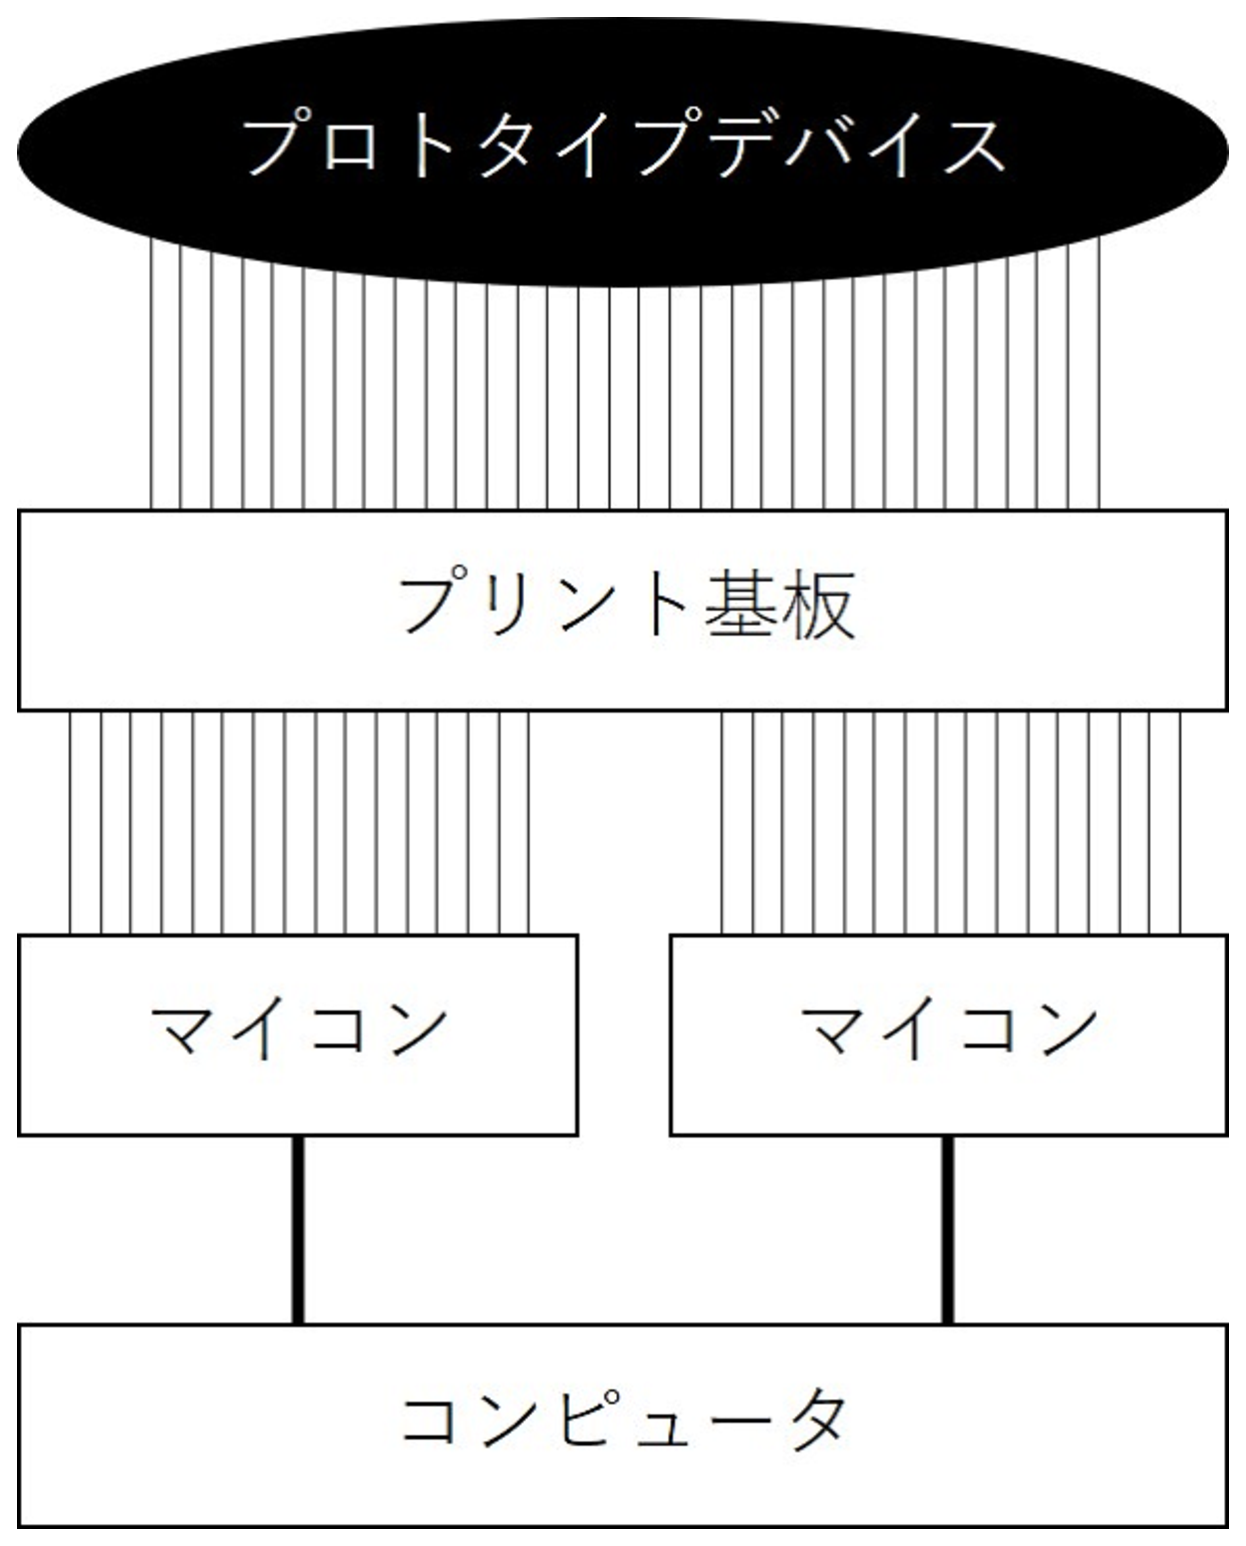
\includegraphics[width=0.5\linewidth]{figure/device.eps}
  \end{center}
  \caption{デバイス構成}
  \label{device}
\end{figure}

\begin{figure}[!t]
  \begin{center}
    \includegraphics[width=0.5\linewidth]{figure/met_over.eps}
  \end{center}
  \caption{プロトタイプデバイスの全体図}
  \label{met_over}
\end{figure}

\begin{figure}[!t]
  \begin{center}
    \includegraphics[width=0.5\linewidth]{figure/met_in.eps}
  \end{center}
  \caption{プロトタイプデバイスの内部}
  \label{met_in}
\end{figure}

\begin{figure}[!t]
  \begin{center}
    \includegraphics[width=0.5\linewidth]{figure/sensor.eps}
  \end{center}
  \caption{センサの実装方法}
  \label{sensor}
\end{figure}

\begin{figure}[!t]
  \begin{center}
    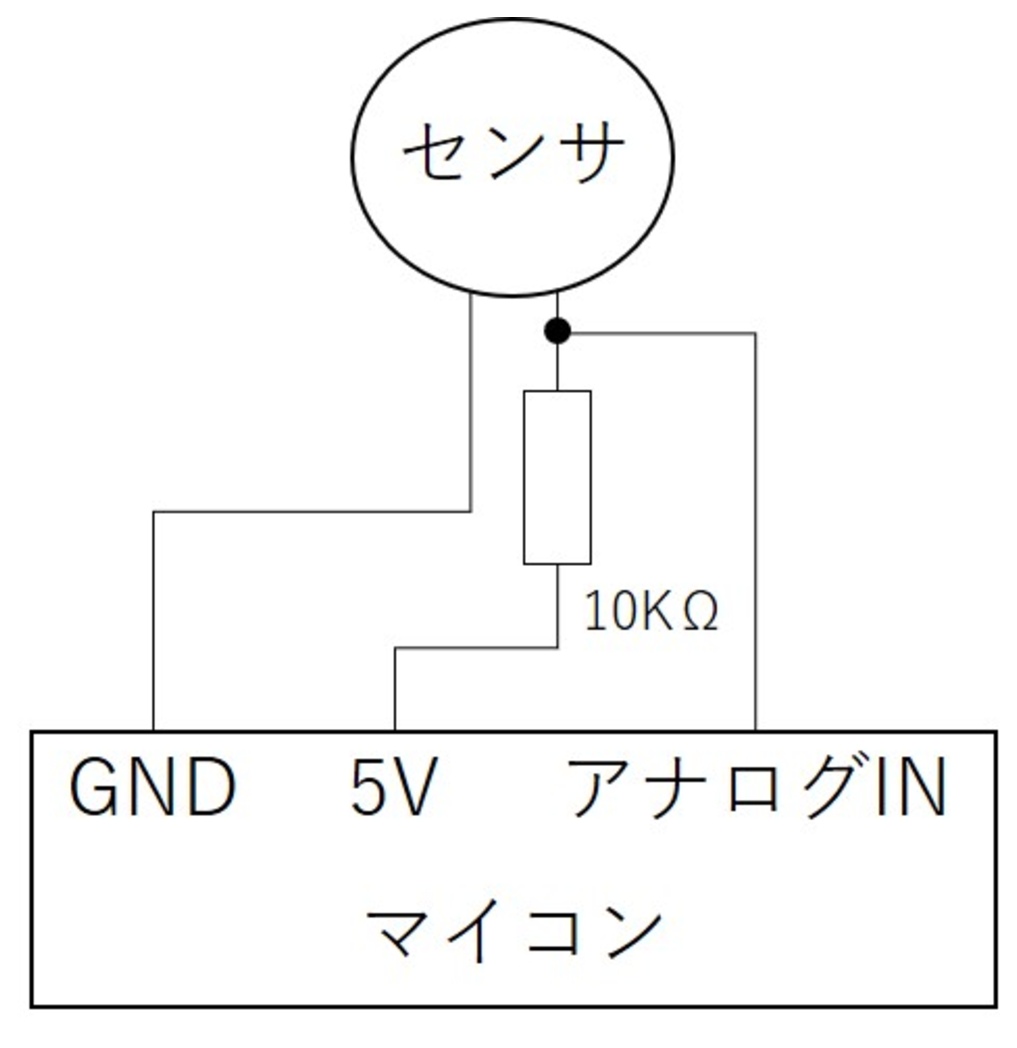
\includegraphics[width=0.5\linewidth]{figure/circuit.eps}
  \end{center}
  \caption{センサ1つあたりの回路図}
  \label{circuit}
\end{figure}

\begin{figure}[!t]
  \begin{center}
    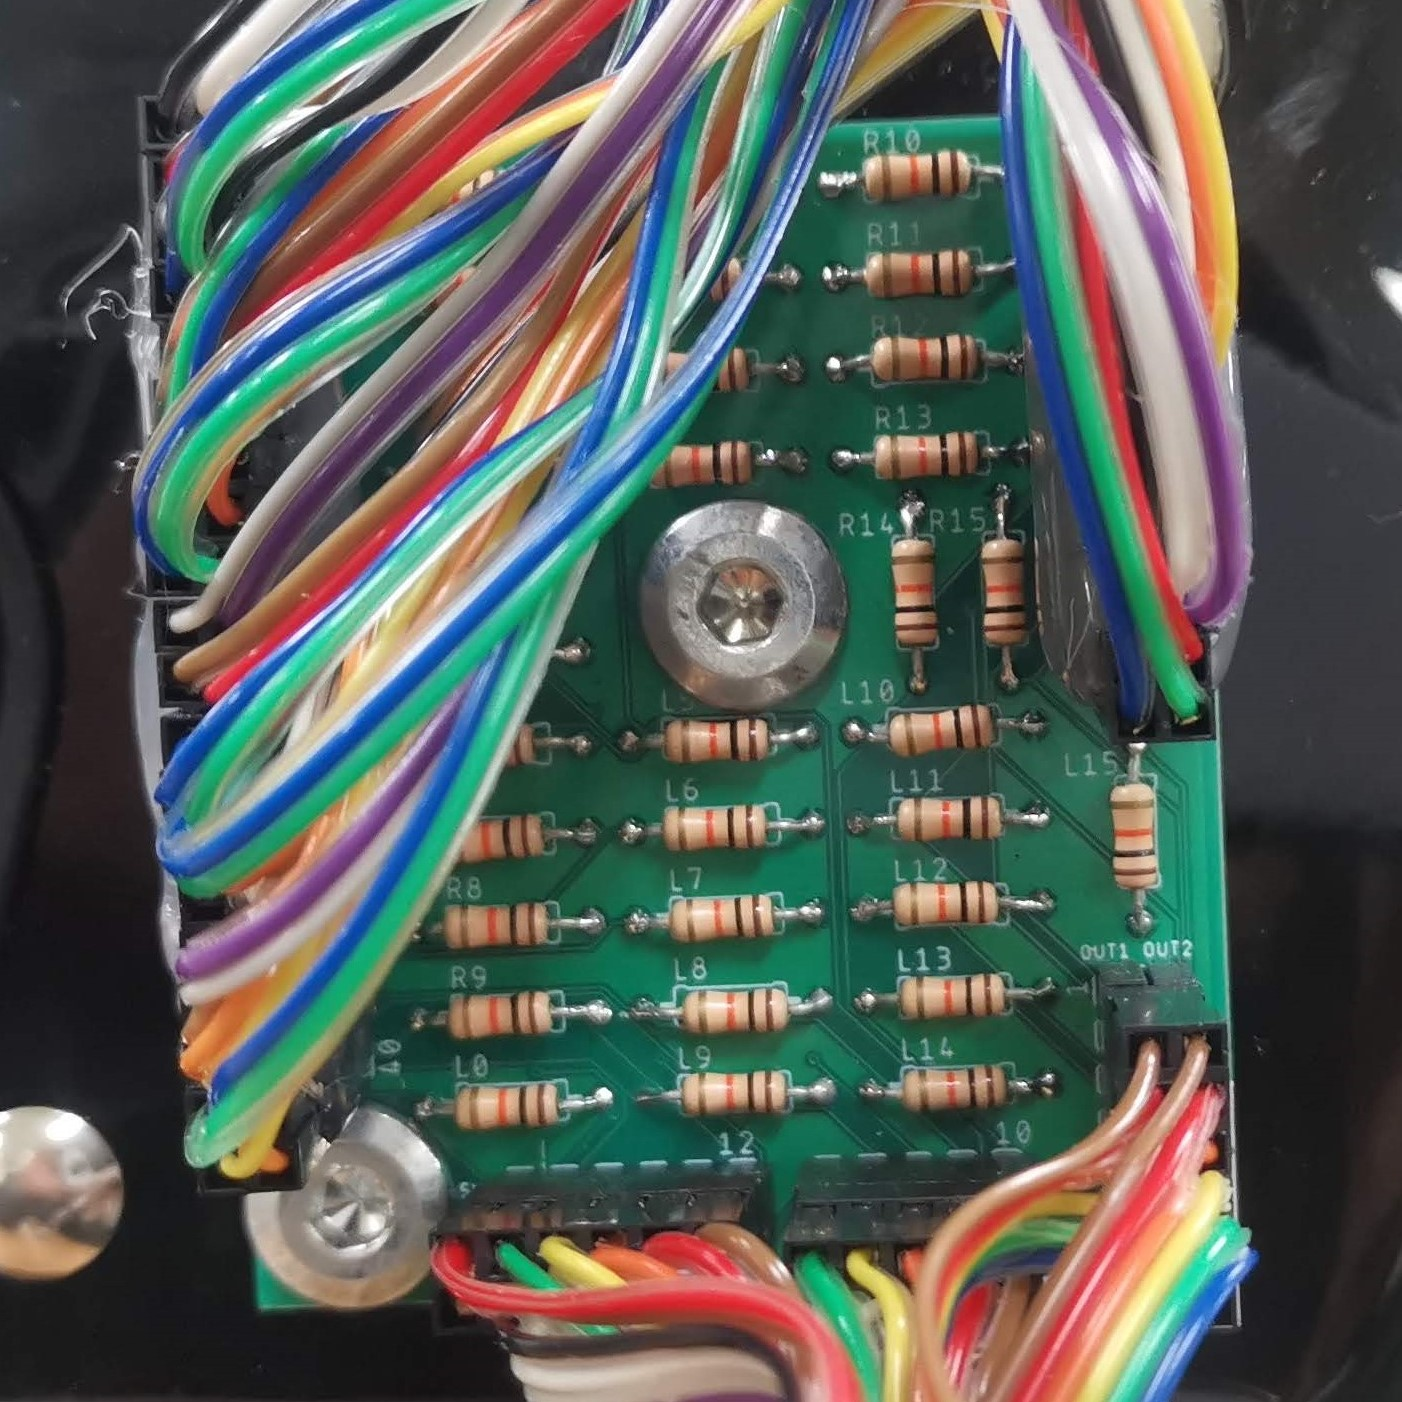
\includegraphics[width=0.5\linewidth]{figure/print.eps}
  \end{center}
  \caption{プリント基板}
  \label{print}
\end{figure}

\subsection{ソフトウェア}
データの収集にはArduinoIDEを用いてマイコンを制御し,Pythonでセンサデータをコンピュータ上にcsvとして収集するプログラムを作成した.次にデータの解析はPython上でcsvを読み出し,sklearn.covariance.MinCovDetを用いてマハラノビス距離を計算した.そして,計算結果に対し閾値を移動させながら比較,識別しながら評価指標を計算するプログラムを実装した.\par
ここで用いたsklearn.covariance.MinCovDetとは,異常値に対して頑健な共分散行列の推定アルゴリズムであるMinimum Covariance Determinant(以下MCDと表記)を高速化したFast-MCD\cite{fast_mcd}を実装したscikit-learnのライブラリである.

%次節でFast-MCDのアルゴリズムについて論じる.
\begin{comment}
文字数水増し
\subsection{Fast-MCDのアルゴリズム}
マハラノビス距離は平均値ベクトルを用いて計算するため,異常値の影響を大きく受けてしまう.そこで,異常値に対して頑健な共分散行列の推定アルゴリズムであるMCDが存在する.しかし,このアルゴリズムは膨大な計算量が必要である.そのため,実際に使えるように高速化されたアルゴリズムがFast-MCDである.Fast-MCDのアルゴリズムは次の通りである.\par
$x_i$を$p$次元の確率ベクトルとしたとき,$X = {x_1, \ldots, x_n}$とし,$H_{old}\subset X$を$X$からランダムに抽出した大きさ$h$の$x_i$の集合とする.まず,$H_{old}$の平均ベクトルと共分散行列をそれぞれ$\hat{\mu}_{old}, \hat{\Sigma}_{old}$とし,$\hat{\Sigma}_{old}$の固有値$|\hat{\Sigma}_{old}|$を計算する.次に$\hat{\mu}_{old}, \hat{\Sigma}_{old}$を使ったマハラノビス距離を$X$の各要素に対して計算し,
\[
d(x_i) = \sqrt{(x_i-\hat{\mu}_{old})^{T}\hat{\Sigma}_{old}^{-1}(x_i-\hat{\mu}_{old})}
\]
とする.$d(x_i)$を小さいもの順に並べ,$d_{j:n}$をその中で$j$番目に大きいものとすると,次のようになる.
\[
d_{1:n}\leq \cdots\leq d_{j-1:n}\leq d_{j:n}\leq d_{j+1:n}\leq \cdots\leq d_{n:n}
\]
ここで,$d_{j:n}$を小さいもの順に$h$個取り出し
\[
H_{new} = {d_{1:n}, d_{2:n}, \ldots, d_{h:n}}
\]
とし,この$H_{new}$の平均ベクトル,共分散行列とその固有値$\hat{\mu}_{new}, \hat{\Sigma}_{new}, |\hat{\Sigma}_{new}|$を計算する.この作業を$|\hat{\Sigma}_{new}|=0$となる,もしくは$|\hat{\Sigma}_{old}|-|\hat{\Sigma}_{new}|$が十分小さくなるまで繰り返す.この一連の流れから得られた平均ベクトルと共分散行列が,異常値に対して頑健なMCD推定量となる.
\end{comment}

\section{評価}
\label{evaluation}
\subsection{データ収集}
提案手法の有効性を確認するために,被験者9名(A$\sim$E,全員男性,平均年齢23歳)にプロトタイプデバイスを着用させ,サンプリングレート約30Hzでセンサデータを収集した.2秒間着用して取り外し,再び着用する試行を1セットとして被験者1人あたり計10セット(2秒$\times$20回分)を収集した.データ収集は1人当たり1 日最大4 セットとし,複数日に渡って実施した.センサと頭部のさまざまな位置関係のデータを収集するために,セット間に30 分以上の休憩時間を設けた.合計で2秒×10セット×9名=360秒のデータを収集した.今回の実験では1度の着用に対して1つのデータが必要なので,1回で収集した2秒間の平均値を解析に使用した.

\subsection{データ群の散らばり}
提案手法は距離に基づき装着者を識別する.すなわち,被験者ごとのデータ群に散らばりがなければ提案手法は成立しない.そのため,収集したすべてのデータに対して主成分分析を行い,2次元に圧縮したデータを2次元平面上にプロットし,目視で確認できるようにした.その結果を図\ref{PCA}に示す.\par

\begin{figure}[!t]
  \begin{center}
    \includegraphics[width=1\linewidth]{figure/PCA.eps}
  \end{center}
  \caption{PCAによる分析結果}
  \label{PCA}
\end{figure}

被験者A,Eのデータ群は分散が小さく,他の被験者のデータ群と重なりも見られない.被験者B,Iのデータ群は分散が小さいものの,互いに重なりが見られる.被験者Cのデータ群は分散が大きいが,1つのデータが被験者Iのデータ群に近い位置にあることを除き,他の被験者のデータ群との重なりは見られない.被験者D,Hのデータ群は分散が小さいが,互いにかなり重なっている.被験者F,Gのデータ群は分散が大きいものの,他の被験者のデータ群との重なりは見られない.\par
以上の結果は2次元に主成分分析しているため,データ量が大きく損失している.その点を考慮した上で,ヘルメット内部に搭載した圧力センサのデータから,距離に基づき装着者を識別できると判断した.

\subsection{提案手法での識別結果}
識別結果の評価指標として,FRR,FAR,EERを用いる.FRR(False reject rate:本人棄却率)は本人のデータを他人と誤って拒否してしまうことであり,FAR(False accept rate:他人受入率)とは他人のデータを本人と誤って認証してしまうことである.閾値を小さくするほどFRRが増加し,閾値を大きくするほどFARが増加する.これらはトレードオフの関係であり,FRRとFARが同値になるときの値をEER(Equal error rate:等価エラー率)と呼ぶ。このEERが小さいほど認証精度が良いとされる.\par
データセットに対し,被験者ごとに提案手法を用いて識別し評価指標を計算する.5分割交差検証を行って識別したときのFRRとFARの結果を図\ref{EER}に,EERの値を表\ref{EER_num}に示す.Totalは被験者全員の平均EERの値を示している.

\begin{figure}[!t]
  \begin{center}
    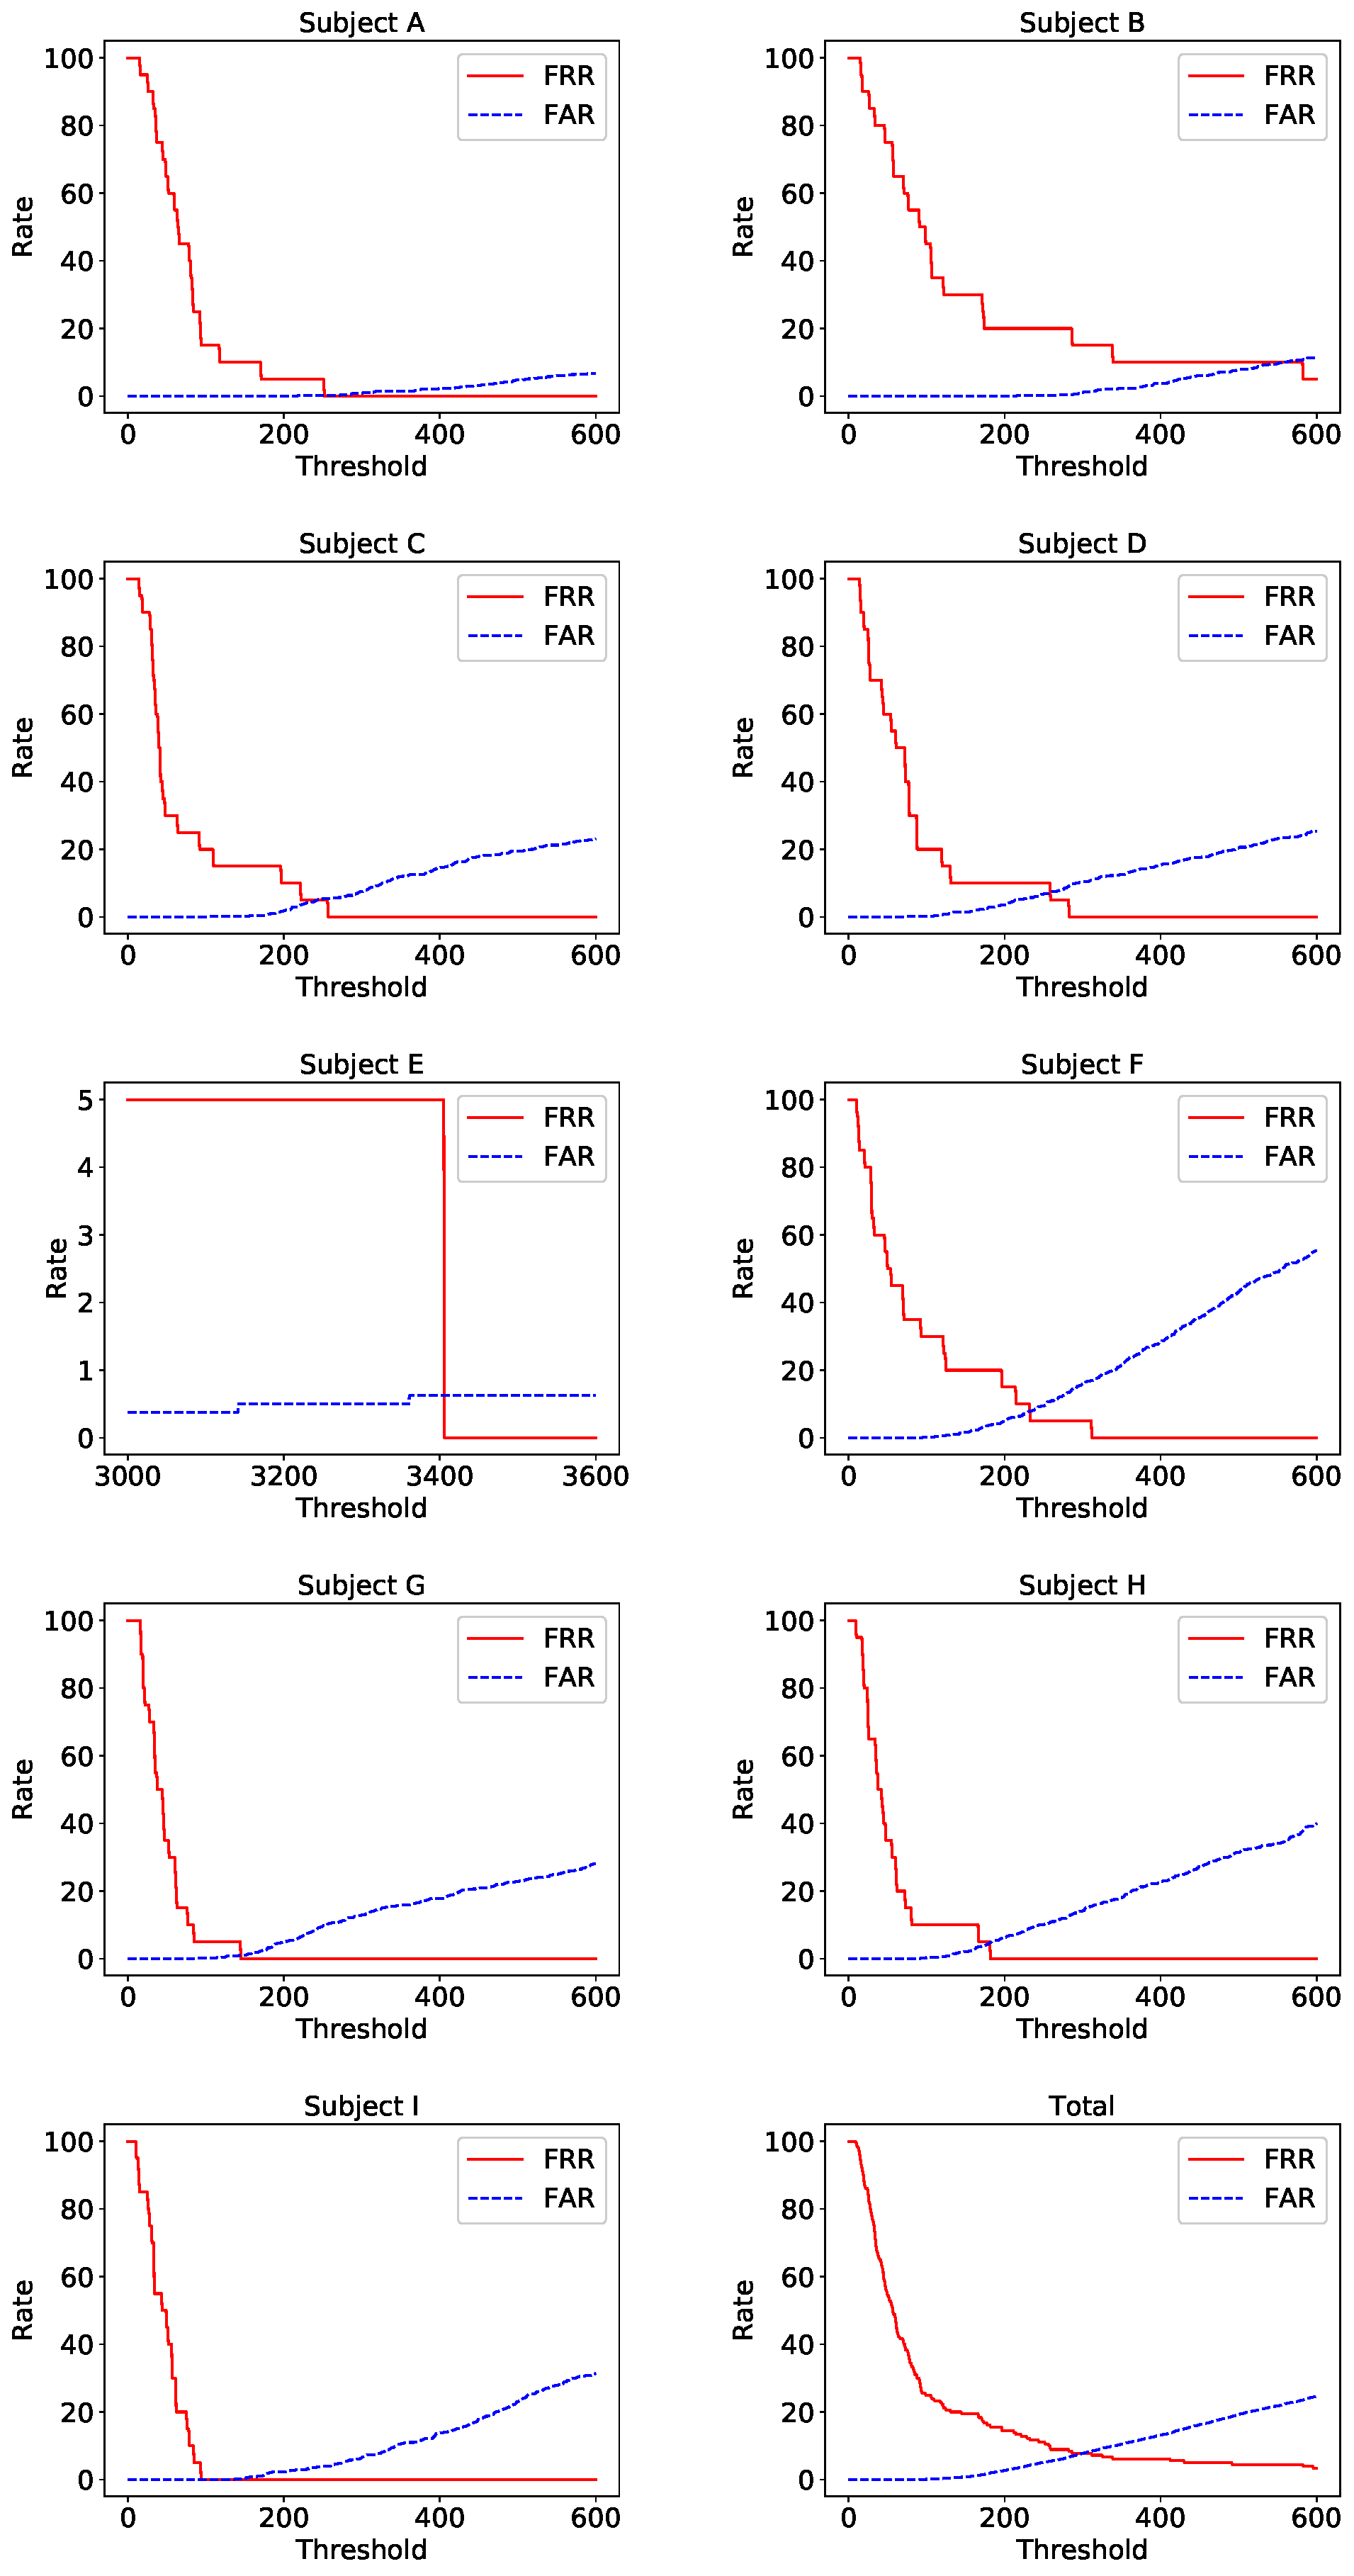
\includegraphics[width=1\linewidth]{figure/EER.eps}
  \end{center}
  \caption{被験者ごとの判別結果}
  \label{EER}
\end{figure}

\begin{table}[htb]
  \centering
  \caption{被験者ごとのEER}
  \begin{tabular}{|c|c|} \hline
    被験者 & EER(\%) \\ \hline \hline
    A & 0.1 \\
    B & 10.0 \\
    C & 5.0 \\
    D & 7.3 \\
    E & 0.6 \\
    F & 7.9 \\
    G & 1.1 \\
    H & 4.6 \\
    I & 0.0 \\ \hline
    Total & 7.8 \\ \hline
  \end{tabular}
  \label{EER_num}
\end{table}

\subsection{識別結果の考察}
表\ref{EER_num}より被験者A,IのEERはほぼ0\%である.これは,検証に用いたデータセットでの識別が概ね完全にできたということを意味している.しかし,図\ref{PCA}では被験者Aと他の被験者のデータ群には重なりがなかったが,被験者Iは重なりが見られる.これは2次元に圧縮した際のデータの損失による影響だと考えられる.次いで結果が良かった被験者EのEERは約0.6\%だった.図\ref{PCA}より,被験者Eのデータ群はかなり隔離されていることが確認できる.しかし,図\ref{EER}を見ると,被験者EのみEERが得られた閾値が大きかったことがわかった.これも同様にデータの損失の影響であり,主成分分析で丸められているが生データでは外れ値が存在したため,FRRが下がりきる閾値が大きくなったと考えられる.他の被験者でも同様に,図\ref{PCA}のデータ群の重なりから予想されるEERと結果が異なる場合があったが,いずれもデータの損失による影響だと考えられる.また,被験者全員の平均EERは約7.8\%という結果であった.被験者ごとのEERに差が見られたことから,さらなる精度の向上を目指すことが可能であると考えられる.\par
提案手法ではマハラノビス距離を用いて識別を行うため,学習データ数をさらに増やすことで精度の向上が見込まれる.一方で,距離が同じ場合は識別が不可能となってしまう.その場合,提案手法と別の手法で識別を行う必要がある.具体的には,ヘルメットを装着する一連の流れを時系列データとして取得し,その特徴により識別を行う手法が考えられる.この手法が有効であるかを今後検証していく.

\section{おわりに}
\label{conclude}
本研究では,圧力センサを内部に取り付けたヘルメットを着用することで頭部の形状を計測し,頭部形状の個人差から二輪車の所有者本人を識別する手法を提案した.評価実験を行うため,プロトタイプデバイスとデータ収集および解析プログラムを作成した.プロトタイプデバイスは市販のフルフェイス型ヘルメットを加工し,圧力センサを取り付けた.このプロトタイプデバイスからデータを取得するためにデータ収集プログラムを作成し,被験者9名から合計で360秒間の頭部形状データを取得した.解析に用いたプログラムはPythonで実装し,sklearn.covariance.MinCovDetでマハラノビス距離を計算,閾値を移動させて装着者の識別を行った.評価実験の結果,認証の精度の評価指標であるEERが個人ごとには約0\%$\sim$約10\%,全体では約7.8\%という結果が得られた.この結果より,本手法は個人識別手法として有効であると考えられる.今後はさらなるデータ収集を行い,実環境での提案手法の評価を行う.また,利用者のデータ群に差がないときの個人識別方法を定義し,検証していく.

\bibliography{references}
\bibliographystyle{junsrt}

\end{document}
